\documentclass[12pt]{article}

\usepackage{setspace}
\usepackage{amsmath,amssymb}
\usepackage{amsfonts}
\usepackage{graphicx}
\newcommand{\lik}{\mathcal{L}}
% \usepackage[toc]{glossaries}
% \makeglossaries
\usepackage[pdftex,bookmarks=true,bookmarksopen=false,bookmarksnumbered=true,colorlinks=true,linkcolor=black]{hyperref}
% \usepackage{biblatex}

\usepackage[utf8]{inputenc}
\usepackage{float}
\usepackage{pdfpages}
\usepackage{tocbibind}
\usepackage{listings}
\usepackage{xcolor}
\usepackage[shortlabels]{enumitem}
\setlength{\parindent}{0em}

\definecolor{codegreen}{rgb}{0,0.6,0}
\definecolor{codegray}{rgb}{0.5,0.5,0.5}
\definecolor{codepurple}{rgb}{0.58,0,0.82}
\definecolor{backcolour}{rgb}{0.95,0.95,0.92}

\lstdefinestyle{mystyle}{
    backgroundcolor=\color{backcolour},   
    commentstyle=\color{codegreen},
    keywordstyle=\color{magenta},
    numberstyle=\tiny\color{codegray},
    stringstyle=\color{codepurple},
    basicstyle=\ttfamily\footnotesize,
    breakatwhitespace=false,         
    breaklines=true,                 
    captionpos=b,                    
    keepspaces=true,                 
    numbers=left,
    numbersep=5pt,                  
    showspaces=false,                
    showstringspaces=false,
    showtabs=false,                  
    tabsize=2,
    inputencoding=utf8,
    extendedchars=true,
    literate={á}{{\'a}}1 {à}{{\`a}}1 {ã}{{\~a}}1 {é}{{\'e}}1 {ê}{{\^e}}1 {ë}{{\"e}}1 {í}{{\'i}}1 {ç}{{\c{c}}}1 {Ç}{{\c{C}}}1 {õ}{{\~o}}1 {ó}{{\'o}}1 {ô}{{\^o}}1 {ú}{{\'u}}1
}

\lstset{style=mystyle}
\renewcommand{\lstlistingname}{Algoritmo}
\usepackage[brazil]{babel}
\usepackage{hyperref}
\usepackage{mathtools}
\usepackage{subfig}
\usepackage{csquotes}
\DeclarePairedDelimiter\ceil{\lceil}{\rceil}
\DeclarePairedDelimiter\floor{\lfloor}{\rfloor}
%\usepackage{pstricks}%, egameps}
\DeclareMathOperator*{\argmin}{arg\,min} % thin space, limits underneath in displays
\DeclareMathOperator*{\argmax}{arg\,max} % thin space, limits underneath in displays
%\setlength{\textwidth}{17.2cm}
% \setlength{\textheight}{23cm}
%\addtolength{\oddsidemargin}{-22mm} 
%\addtolength{\topmargin}{-15mm} \addtolength{\evensidemargin}{-15mm}
%\setlength{\parskip}{1mm}
%\setlength{\baselineskip}{500mm}

\newtheorem{theorem}{Theorem}[section]
\newtheorem{assumption}{Assumption}
\newtheorem{acknowledgment}{Acknowledgment}
\newtheorem{algorithm}{Algorithm}
\newtheorem{axiom}{Axiom}
\newtheorem{case}{Case}
\newtheorem{claim}{Claim}
\newtheorem{conclusion}{Conclusion} 
\newtheorem{condition}{Condition}
\newtheorem{conjecture}{Conjecture}
\newtheorem{corollary}{Corollary}[section]
\newtheorem{criterion}{Criterion}
\newtheorem{defn}{Definition}[section]

\newtheorem{example}{Example}[section]
\newtheorem{exercise}{Exercise}
\newtheorem{lemma}{Lemma}[section]
\newtheorem{notation}{Notation}
\newtheorem{problem}{Problem}
\newtheorem{proposition}{Proposition}[section]
\newtheorem{remark}{Remark}
\newtheorem{solution}{Solution}
\newtheorem{summary}{Summary}
\newenvironment{proof}[1][Proof]{\textbf{#1.} }{\rule{0.5em}{0.5em}}

% \newglossaryentry{maths}
% {
%     name=mathematics,
%     description={Mathematics is what mathematicians do}
% }

\newpage 

\begin{document}

\begin{titlepage}
\begin{center}
\textbf{\LARGE Fundação Getúlio Vargas}\\ 
\textbf{\LARGE Escola de Matemática Aplicada}

\par
\vspace{160pt}
\textbf{\Large Rener Oliveira}\\
\vspace{160pt}
\textbf{\Large Inferência Estatística Trabalho 2: Algoritmo EM}\\

\end{center}
\vspace{32pt}
\par
\vfill
\vspace{32pt}
\begin{center}
{\normalsize Setembro de 2020}
\end{center}
\end{titlepage}

\newpage
\tableofcontents



%------------------------>>>>>>>>>>Começaremos por aqui
%\newpage
% \addcontentsline{toc}{section}{Introdução} \section*{Introdução}


\newpage


\section{O Algoritmo}

\subsection{Glossário (Notações)}
\begin{itemize}
    \item $\vec{X}$: Dados observados;
    \item $\vec{Z}$: Dados faltantes;
    \item $\Omega$: Espaço de parâmentros;
    \item $\theta^{(j)}$: Estimador de $\theta$ na iteração $j$ do algoritmo EM;
    \item $\lik(\theta;\vec X,\vec Z)$: Verossimilhança dos dados completos;
    \item $\lik(\theta;\vec X)$: Verossimilhança dos dados observados (incompletos);
    \item $f(x,z|\theta)$: Distribuição conjunta dos dados completos ($f(x,z|\theta)=\lik(\theta;\vec X,\vec Z)$);
    \item $g(x|\theta)$: Distribuição dos dados observados ($g(x|\theta)=\lik(\theta;\vec X)$).
\end{itemize}
 
O Estimador de Máxima Verossimilhança (EMV) em muitas situações práticas pode ser difícil de ser computado. Um exemplo recorrente é quando temos em nossa amostra um subconjunto de dados faltantes \textit{("missing data")}; 

Uma solução pra esse problema é o famoso Algoritmo EM\cite{degroot2012probability}\cite{wiki_exp} (\textit{"Expectation-Maximization"}) que é uma método iterativo para aproxima o EMV nessas situações de dados faltantes.

De forma geral, queremos um estimador para o vetor de parâmetros $\theta\in\Omega$ $\lik (\theta;\vec X)$.

$\displaystyle\hat{\theta}_{EMV}=\argmax_{\theta \in \Omega} \lik (\theta;\vec X)$

Mas $\displaystyle\lik (\theta;\vec X) = \int f(x,z|\theta)d\vec Z$ e não iremos trabalhar com a maximização direta dessa integral, mas usaremos o seguinte processo iterativo:


\begin{itemize}
    \item Passo "E": Dado um $\theta^{(j)}$, o passo \textit{Expectation}, consiste em "eliminar" de certa forma a lacuna dos dados faltantes, usando o valor esperado da log-verossimilhança dos dados completos com respeito a $\theta^{(j)}$\footnote{Como condição inicial $\theta^{(0)}$ podemos pegar qualquer vetor de $\Omega$} e $\vec X$. Ou seja, definimos uma função $Q(\theta|\theta^{(j)})$, onde:
    
    $$Q(\theta|\theta^{(j)})=E[\ln \lik (\theta;\vec X, \vec Z)|\theta^{(j)},\vec X]$$
    
    \item Passo "M": inicial de \textit{Maximization} este passo consiste em encontrar o valor que maximiza a função acima. Este valor será plugado como $\theta^{(j+1)}$ e a iteração continuará. Formalmente:\cite{wiki_exp}
    
    $$\theta^{(j+1)}=\argmax_{\theta\in\Omega}Q(\theta|\theta^{(j)})$$
    
\end{itemize}


De fato, não é difícil mostrar que 

$$\lik(\theta|\vec X)\geq Q(\theta|\theta^{(j)}) = E[\ln \lik (\theta;\vec X, \vec Z)|\theta^{(j)},\vec X],$$

as notas de \cite{bin} mostram isso para o caso discreto e o artigo \cite{singh2005algorithm} usa este fato para o caso contínuo. Tendo essa desigualdade, é fácil ver que o algoritmo ao maximizar $Q(\theta|\theta^{(j)})$ está maximizando $\lik(\theta|\vec X)$ que é nosso objetivo. Daremos mais detalhes na seção de demonstração da monotonicidade do método.





\section{Exemplo das Moedas}

\textbf{Problema (Transcrição):}

Suponha que temos duas moedas, Moeda 1 e Moeda 2 de modo que $Pr(Cara|Moeda = 1) =p_1$ e $Pr(Cara|Moeda =2) =p_2$; Suponha agora que fazemos o seguinte experimento:

\begin{enumerate}[(i)]
    \item Selecionamos uma moeda aleatoriamente com probabilidade $1/2$;
    \item Lançamos a moeda selecionada $m$ vezes;
    \item Repetimos (i) e (ii) $n$ vezes.
\end{enumerate}

Podemos representar os dados advindos deste experimento como:

$$\begin{matrix} X_{11}&...&X_{1m}&~&M_1\\
 X_{21}&...&X_{2m}&~&M_2\\
 \vdots &...&\vdots &~&\vdots\\
  X_{n1}&...&X_{nm}&~&M_n
\end{matrix}$$

onde os $X_{ij}$ são variáveis de Bernoulli que guardam o resultados do lançamento da moeda e $M_i\in \{1,2\}$ é a variável aleatória que guarda qual moeda foi selecionada na $i$-ésima rodada do experimento.

Desenvolveremos aqui um esquema EM para aproximar o EMV de $\theta=(p_1,p_2)$ quando desconhecemos os valores de $M_i$.

Este é um problema clássico, conhecido como Binomial Mixture \cite{bin}, na qual se tem um conjunto de tipos de moedas com probabilidades de dar cara diferentes, seleciona-se uma dessas moedas e realizam-se experimentos binomiais (bernoulli repetidamente). No final, ficamos com o conjunto de observações dos resultados, mas não sabemos qual tipo da moeda que gerou cada resultado, e o objetivo da aplicação do método EM é estimar o vetor de probabilidades dos tipos da moeda.

Nosso problema é um caso particular da referência \cite{bin}, pois temos apenas dois tipos de moedas, e a probabilidade de escolher uma ou outra é igual a $1/2$. O caso geral é bem interessante, pois além de explorar uma quantidade variável de experimentos a cada rodada (aqui temos fixo $m$) ele explora também o desconhecimento das probabilidades de escolha entre os tipos da moeda, que passam a incorporar o vetor de parâmetros a ser estimado.

Seguem algumas definições que usaremos:

\textbf{Notações e Definições}
\begin{itemize}
    \item $\theta_i$: $p_1$ se $M_i=1$, ou $p_2$ se $M_i=2$;
    \item $S_i=\sum_{j=1}^mX_{ij}$, neste caso, $S_i$ tem distribuição binomial de parâmetros $m$ e $\theta_i$;
    \item $\vec X$: Vetor de dados incompletos $(S_1,\,...\,,S_n)$ 
    \item $\vec M = (M_1,\,...\,,M_n)$ (dados faltantes)
\end{itemize}

O que estamos fazendo é sumarizando a informação matricial dos experimentos em um vetor que contem a quantidade de caras de cada experimento. Este vetor será composto por distribuições binomiais, e tiraremos proveito disso para derivar a fórmula iterativa de $\theta^{(r)}$.

O processo que seguiremos para aproximar o EMV de $\theta$ é o seguinte:

\begin{itemize}
    \item Escolher $\theta^{(0)}$ qualquer em $\in (0,1)\times (0,1)$;
    \item (Passo E)Computamos a função $Q(\theta,\theta^{(j)})=E[\ln \lik (\theta;\vec X, \vec M)|\theta^{(j)},\vec X]$
    \item (Passo M) Escolhemos $\displaystyle \theta^{(j+1)} = \argmax_{\theta\in\Omega}Q(\theta|\theta^{(j)})$
    \item Repetimos os dois itens anteriores até a condição de parada, que pode ser, atingimento de tolerância, $|\theta^{(j+1)}-\theta^{(j)}|<\varepsilon$, para algum $\varepsilon$ inicialmente definido, ou quando um número máximo de iterações pré-definido é atingido.
\end{itemize}

Para realizar os passos E e M, vamos derivar a função $Q(\theta,\theta^{(j)})$ explicitamente.

\subsection{Passo E}

Primeiramente vamos escrever a verossimilhança dos dados completos.

Para cada $i$, temos\footnote{Como $\vec X = (S_1,\,...\,,S_n)$, definiremos $X_i=S_i$ para todo $i$ de 1 a $n$}

$P(X_i,M_i|\theta)\\$

\footnote{Probabilidade Condicional $\displaystyle P(A,B|C)=P(A|B,C)\cdot P(B|C)$}$=P(X_i|M_i,\theta)\cdot P(M_i|\theta)\\ =\dfrac12\cdot P(X_i|M_i,\theta)\\$

Como $X_i=S_i$ é binomial de parâmetros $m$ e $\theta_i$, temos que:

$\\ \displaystyle P(X_i,M_i|\theta) = \frac12\cdot Bin(X_i,\theta_i),\\$

onde $\displaystyle Bin(X_i,\theta_i) = \binom{m}{S_i}\theta_i^{S_i}(1-\theta_i)^{m-S_i}$. Estamos usando uma notação similar\footnote{Na verdade estamos cometendo um abuso de notação usando $ Bin(X_i,\theta_i)$ como função que é igual a probabilidade de uma binomial $(m,\theta_i)$ ser igual a $X_i$} às notas de \cite{bin}, porém omitimos o $m$ de $Bin(X_i|m,\theta_i)$ pois no nosso caso é uma valor fixo para todo $i$.

Dessa forma, a verossimilhança será:

$\displaystyle\lik (\theta;\vec X, \vec M) = \prod_{i=1}^nP(X_i,M_i|\theta)=\\
\prod_{i=1}^n\frac12 Bin(X_i,\theta_i)$

Tomando o logaritmo natural (log do produto é a soma dos logs), teremos:

$\displaystyle\ln \lik (\theta;\vec X, \vec M) = n\ln\frac12+\sum_{i=1}^n\ln Bin(X_i,\theta_i)$

Temos então, por definição:

$\displaystyle Q(\theta,\theta^{(j)}) = E[\lik (\theta;\vec X, \vec M)|\vec X,\theta^{(j)}]\\=E\left[\left.n\ln\frac12+\sum_{i=1}^n\ln Bin(X_i,\theta_i)\right|\vec X,\theta^{(j)}\right]\\
n\ln\frac12+\sum_{i=1}^nE[\ln Bin(X_i,\theta_i)|\vec X,\theta^{(j)}]$

Finalizamos então a etapa \textit{Expectation}, computando a função $Q$:

\begin{equation}
    \label{eqn:qfun}
    \displaystyle Q(\theta,\theta^{(j)}) = n\ln\frac12+\sum_{i=1}^nE[\ln Bin(X_i,\theta_i)|\vec X,\theta^{(j)}]
\end{equation}

\subsection{Passo M}

Vamos agora, maximizar a função acima. Usaremos derivação, ao fazer isso estamos supondo algumas condições de regularidade na função $Q$, mas isso será melhor detalhado na seção seguinte. Por enquanto, vamos aceitar que podemos fazer isso sem problemas.

Nosso objetivo nessa etapa é, encontrar:

$$\theta^{(j+1)}=\argmax_{\theta\in(0,1)^2}\left(n\ln\frac12+\sum_{i=1}^nE[\ln Bin(X_i,\theta_i)|\vec X,\theta^{(j)}]\right)$$

Mas como $n\ln\frac12$ não depende de $\theta$, a expressão acima é igual a:

$$\argmax_{\theta\in(0,1)^2}\left(\sum_{i=1}^nE[\ln Bin(X_i,\theta_i)|\vec X,\theta^{(j)}]\right)$$

O processo de maximização consiste em computar $\theta_1$ e $\theta_2$ tal que $\partial Q/\partial \theta_1 =0$
e $\partial Q/\partial \theta_2 =0$; teremos então o vetor $\theta^{(j+1)}=(\theta_1,\theta_2)$

Vamos calcular, por simplicidade, apenas $\partial Q/\partial \theta_1$, e veremos que o processo para $\theta_2$ é completamente análogo.

Como vimos acima, o argmax de Q foi reduzimo para um expressão mais simples. Vamos trabalhar então com a derivada dessa expressão:

$$\dfrac{\partial}{\partial \theta_1}\left(\sum_{i=1}^nE[\ln Bin(X_i,\theta_i)|\vec X,\theta^{(j)}]\right)=\sum_{i=1}^n\dfrac{\partial}{\partial \theta_1}E[\ln Bin(X_i,\theta_i)|\vec X,\theta^{(j)}]$$

Note que, fixado $i$, o termo $E[\ln Bin(X_i,\theta_i)|X_i,\theta^{(j)}]$\footnote{Note que trocamos $\vec X$ por $X_i$ pois pela independência dos experimentos, o único elemento do vetor $\vec X$ com informações de interesse é $X_i=S_i$.}pode ser escrito como:

\begin{equation}
    \label{eqn:deriv}
\ln[Bin(X_i,\theta_1)]\cdot P(M_i=1|X_i,\theta^{(j)})+\ln[Bin(X_i,\theta_2)]\cdot P(M_i=2|X_i,\theta^{(j)}),\end{equation}


na qual, pela definição de probabilidade conjunta condicional, temos:

$P(M_i=1|X_i,\theta^{(j)})=\dfrac{P(M_i=1,X_i|\theta^{(j)})}{P(X_i|\theta^{(j)})}=\\
\dfrac{P(M_i=1)P(X_i|\theta^{(j)})}{P(X_i|\theta_1^{(j)})P(M_i=1)+P(X_i|\theta_2^{(j)})P(M_i=2)}$

Mas por hipótese, $P(M_i=1)=P(M_i=2)=\frac12$, assim, cancelamos todos esses termos e obtemos:

$P(M_i=1|X_i,\theta^{(j)})=\dfrac{P(X_i|\theta^{(j)})}{P(X_i|\theta_1^{(j)})+P(X_i|\theta_2^{(j)})}=$
\begin{equation}
    \label{bi1}
    \dfrac{Bin(X_i,\theta_1^{(j)})}{Bin(X_i,\theta_1^{(j)})+Bin(X_i,\theta_2^{(j)})}
\end{equation}


Para fins computacionais\cite{bin}, computaremos a quantidade acima usando seu valor explícito:

\begin{equation}
    \label{eqn:compute}
    P(M_i=1|X_i,\theta^{(j)})=\left[1+\left(\dfrac{\theta_2^{(j)}}{\theta_1^{(j)}}\right)^{X_i}\left(\dfrac{1-\theta_2^{(j)}}{1-\theta_1^{(j)}}\right)^{m-X_i}\right]^{-1}
\end{equation}

Para $P(M_i=2|X_i,\theta^{(j)})$ as expressões são análogas.


Note o termo $P(M_i=1|X_i,\theta^{(j)})$  da expressão (\ref{eqn:deriv}) é constante em relação a $\theta_1$. Note também que a segunda parcela, não dependem de $\theta_1$, logo, ao derivarmos a expressão com respeito a $\theta_1$, teremos:

$\displaystyle\sum_{i=1}^n\dfrac{\partial}{\partial \theta_1}E[\ln Bin(X_i,\theta_i)|\vec X,\theta^{(j)}]
\\
=\sum_{i=1}^n\dfrac{\partial}{\partial \theta_1}\ln[Bin(X_i,\theta_1)]\cdot P(M_i=1|X_i,\theta^{(j)})\\
=\sum_{i=1}^n\dfrac{\partial}{\partial \theta_1}\ln[Bin(X_i,\theta_1)]\cdot \dfrac{Bin(X_i,\theta_1^{(j)})}{Bin(X_i,\theta_1^{(j)})+Bin(X_i,\theta_2^{(j)})}$

Fazendo $B_i=\dfrac{Bin(X_i,\theta_1^{(j)})}{Bin(X_i,\theta_1^{(j)})+Bin(X_i,\theta_2^{(j)})}$, temos:

$\displaystyle\sum_{i=1}^n\dfrac{\partial}{\partial \theta_1}E[\ln Bin(X_i,\theta_i)|\vec X,\theta^{(j)}]\\
=\sum_{i=1}^n\dfrac{\partial}{\partial \theta_1}\ln[Bin(X_i,\theta_1)]\cdot B_i$.

Com alguns cálculos, que omitirei, é possível chegar em:

$\dfrac{\partial}{\partial \theta_1}\ln[Bin(X_i,\theta_1)]=\dfrac{X_i-\theta_1 m}{\theta_1(1-\theta_1)};$

Continuando, teremos a derivada igual a:

$\displaystyle\sum_{i=1}^n \dfrac{X_i-\theta_1 m}{\theta_1(1-\theta_1)}\cdot B_i$

Queremos $\theta_1$ que zere a expressão acima. Note que $\theta_\in(0,1)\Rightarrow \theta_1(1-\theta_1)\neq0$, logo, podemos encontrar tal valor, fazendo:

$\displaystyle\sum_{i=1}^n (X_i-\theta_1 m)B_i=0\Rightarrow\\
\displaystyle\sum_{i=1}^n X_iB_i-\theta_1 m B_i=0\Rightarrow\\
\displaystyle\sum_{i=1}^n X_iB_i-\theta_1 m\displaystyle\sum_{i=1}^nB_i=0\Rightarrow\\
\theta_1=\dfrac{\sum_{i=1}^nX_iB_i}{m\sum_{i=1}^nB_i}$

Onde $B_i=P(M_i=1|X_i,\theta^{(j)})$ que pode ser computado pelas expressões (\ref{bi1}) ou (\ref{eqn:compute}). A expressão acima é o nossa primeira coordenada de $\theta^{(j+1)}$. Para encontrar o segundo valor, os passos e resultados são análogos.


\subsection{Conclusões}

A sequência do método EM será dada por $\theta^{(j+1)}=(\theta_1,\theta_2)$, onde:

$\theta_1=\dfrac{\sum_{i=1}^nX_iB_i}{m\sum_{i=1}^nB_i}$ na qual $B_i$ depende de $\theta^{(j)}$ e é dado por (\ref{bi1}) ou (\ref{eqn:compute}), e

$\\ \theta_2=\dfrac{\sum_{i=1}^nX_iB'_i}{m\sum_{i=1}^nB'_i}$ na qual $B'_i$ é dado por:

$\\ \dfrac{Bin(X_i,\theta_2^{(j)})}{Bin(X_i,\theta_1^{(j)})+Bin(X_i,\theta_2^{(j)})}\\$

ou 

$\\ \left[1+\left(\dfrac{\theta_1^{(j)}}{\theta_2^{(j)}}\right)^{X_i}\left(\dfrac{1-\theta_1^{(j)}}{1-\theta_2^{(j)}}\right)^{m-X_i}\right]^{-1}$


\subsection{Simulação computacional}

Fizemos uma simulação usando Python 3.7.6. Geramos uma tabela de experimentos onde as duas moedas tem probabilidades $p_1=0.3$ e $p_2=0.6$ de dar cara. O valor inicial foi escolhido aleatoriamente e chutou um valor menor que 0.2 para as duas quantidades. Note que apesar de estar próximo de $p_1$, está bem longe de $p_2$.

Usamos $n=300$ e $m=30$, ou seja, 300 experimentos de 30 lançamentos. Por simplicidade de implementação, a condição de parada é apenas um número máximo pré-fixado de iterações, mas o ideal seria implementar uma tolerância para o aumento da log-verossimilhança.

Os resultados são apresentados através de dois gráficos: o primeiro, exibido na Figura (\ref{fig:sim}) compara o método EM com o estimador de máxima verossimilhança de $p_1$ e $p_2$, que foram computados como a proporção de caras em que cada moeda registrou, omitiremos aqui a derivação desse estimador. Podemos ver que com poucas iterações, o método convergiu para o MLE (\textit{"Maximum Likelihod Estimator"}). Além disso, $p1\_MLE\approx 0.3063$ e $p2\_MLE\approx 0.6165$, valores bem próximos dos reais. 

É de se esperar que o método EM convirja também para os valores reais dos parâmetros, que é uma afirmação que se sustenta dada a consistência do MLE da bernoulli/binomial, que não demonstraremos aqui, assim, no limite, o MLE converge em probabilidade para o valor real.

\begin{figure}[!htb]
    \centering
    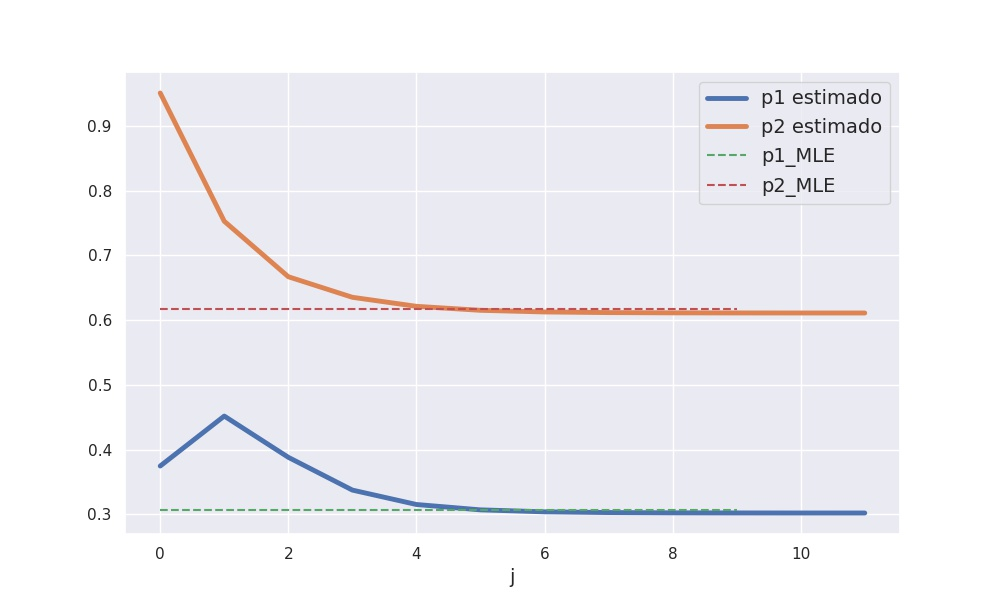
\includegraphics[scale=0.5]{sim2-MLE.jpg}
    \caption{Simulação Método EM vs. MLE(n=300, m=30)}
    \label{fig:sim}
\end{figure}

O segundo gráfico, exibido da Figura (\ref{fig:simr}) é quase idêntico ao citado acima, mas agora o contraste é feito com o valor real dos parâmetros. Note que o método EM superestima o valor de $p_2$, mas isso ocorre pois o próprio MLE faz essa ligeira superestimação; Já que o método EM converge para o MLE, estamos sujeitos à esse tipo de incerteza do próprio MLE.


\begin{figure}[!htb]
    \centering
    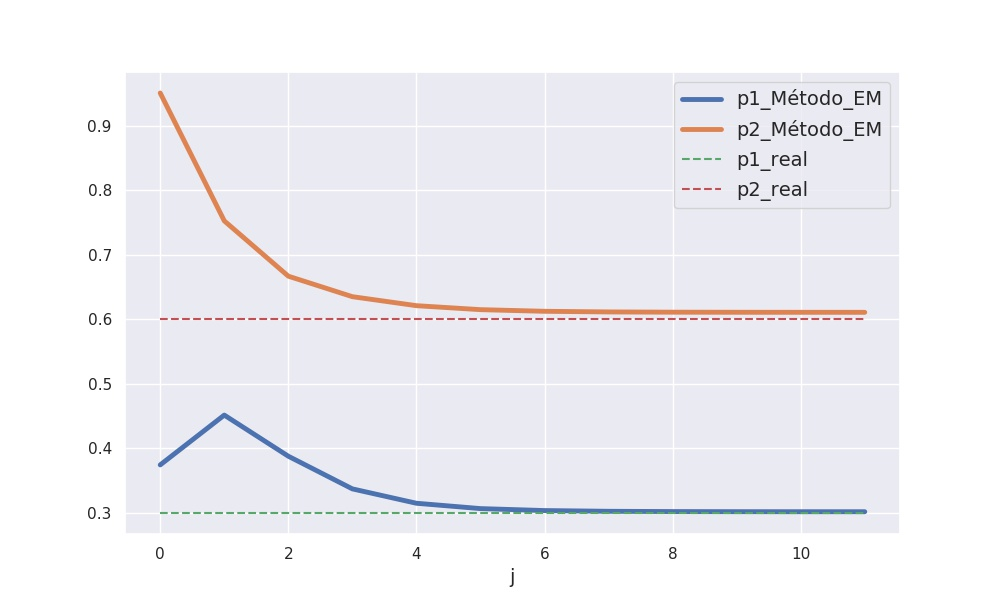
\includegraphics[scale=0.5]{sim2-real.jpg}
    \caption{Simulação Método EM vs. Valor Real(n=300, m=30)}
    \label{fig:simr}
\end{figure}

Note também nas figuras que o valor inicial (aleatório) foi bem distante do valor do MLE do parâmetros, mas o processo iterativo foi muito eficiente, e com poucos passos convergiu, podemos perceber visualmente que após a quinta iteração (j=5) as curvas se aproximam de uma reta.

\newpage
\section{Demonstração da Monotonicidade}

Queremos provar o Teorema 7.2.20 de \cite{CaseBerg:01}:

\textbf{Teorema 7.2.20 (Adaptado):} A sequência $\{\theta^{(j)}\}$ definida como $\displaystyle\theta^{(j+1)}=\argmax_{\theta\in\Omega}Q(\theta|\theta^{(j)})$, onde $Q(\theta|\theta^{(j)})=E[\ln \lik (\theta;\vec X, \vec Z)|\theta^{(j)},\vec X]$ satisfaz:

$$\lik (\theta^{(j+1)};\vec X)\geq \lik (\theta ^{(j)};\vec X)$$

\textbf{Demostração:}

OBS: Usaremos as notações e definições do glossário da seção 1.


Seja $k(z|\theta,x) = \dfrac{f(x,z|\theta)}{g(x|\theta)}$ a distribuição de $\vec Z$ dados $\theta$ e $\vec X$. Sabendo que $\lik (\theta;\vec X,\vec Z)= f(x,z|\theta)$ e $\lik (\theta;\vec X)=g(x|\theta)$, temos que:

$\ln k(z|\theta,x) = \ln \lik (\theta;\vec X,\vec Z)-\ln \lik (\theta;\vec X),$

Logo:

$\ln \lik (\theta;\vec X) = \ln \lik (\theta;\vec X,\vec Z) - \ln k(z|\theta,x) $

Tomando o valor esperado\cite{CaseBerg:01} com respeito à distribuição de $k(z|\theta^{(j)},x)$, o primeiro membro permanecerá como está, pois não há termos de $\vec Z$ livres; Assim teremos:

$\ln \lik (\theta;\vec X) = E[\ln \lik (\theta;\vec X,\vec Z)|\theta^{(j)},\vec X] - E[\ln k(z|\theta,x)|\theta^{(j)},\vec X]$

Vamos definir $H(\theta,\theta^{(j)}):=-E[\ln k(z|\theta,x)|\theta^{(j)},\vec X]$. É chamada de função de entropia\cite{wiki_exp} em outros contextos, mas vamos manter aqui como uma simples definição para simplificação de escrita.

Temos da última equação a seguinte identidade:
\begin{equation}
    \label{eqn:cas_id1}
    \ln \lik (\theta;\vec X) = Q(\theta,\theta^{(j)}) + H(\theta,\theta^{(j)})
\end{equation}

Que vale para todo $\theta$ no espaço de parâmetros, e em particular para $\theta^{(j)}$. Assim, podemos escrever:

$\ln \lik (\theta^{(j)};\vec X) = Q(\theta^{(j)},\theta^{(j)}) + H(\theta^{(j)},\theta^{(j)})$

Como $\theta^{(j+1)}$ é argmax de $Q(\theta,\theta^{(j)})$, temos por definição que $\forall \theta \in \Omega,Q(\theta^{(j+1)},\theta^{(j)})\geq Q(\theta,\theta^{(j)})$. Portanto $Q(\theta^{(j+1)},\theta^{(j)})\geq Q(\theta^{(j)},\theta^{(j)})$, o que prova o item (a) do exercício 7.32 de Casella\cite{CaseBerg_ex}.

Nosso objetivo é provar que $\ln \lik (\theta^{(j+1)};\vec X)\geq \ln \lik (\theta^{(j)};\vec X)$, e pela identidade (\ref{eqn:cas_id1}), Se provarmos que $Q(\theta^{(j+1)},\theta^{(j)})\geq Q(\theta^{(j)},\theta^{(j)})$ (já feito) e $H(\theta^{(j+1)},\theta^{(j)})\geq H(\theta^{(j)},\theta^{(j)})$, o Teorema fica demonstrado.

Resta-nos então provar $H(\theta^{(j+1)},\theta^{(j)})\geq H(\theta^{(j)},\theta^{(j)})$ que é o item (b) do exercícios já citado.

Usando a Desigualdade de Jensen\cite{CaseBerg_jens} para funções côncavas (e a concavidade de $\ln$), podemos mostrar facilmente a dica do item (b) do exercício que afirma que, se $f$ e $g$ são funções de densidade de probabilidade, temos:

\begin{equation}
    \label{eqn:dica}
    \int \ln [f(x)]g(x) dx \leq \int \ln [g(x)]g(x)dx
\end{equation}

Tomemos então $E[\ln k(z|\theta,x)|\theta^{(j)},\vec X]$. Por definição, temos:

$E[\ln k(z|\theta,x)|\theta^{(j)},\vec X] = \displaystyle\int \ln k(z|\theta,x) \ln k(z|\theta^{(j)},\vec X)d\vec Z$

e de (\ref{eqn:dica}), temos:

$\displaystyle\int \ln k(z|\theta,x) \ln k(z|\theta^{(j)},\vec X)d\vec Z\\ \leq \displaystyle\int \ln k(z|\theta^{(j)},\vec X) \ln k(z|\theta^{(j)},\vec X)d\vec Z\\ =E[\ln k(z|\theta^{(j)},\vec X)|\theta^{(j)},\vec X],$

onde a última igualdade vem da definição de esperança condicional.

Com isso, concluímos que 

$\forall \theta \in \Omega;\,E[\ln k(z|\theta,x)|\theta^{(j)},\vec X]\leq E[\ln k(z|\theta^{(j)},\vec X)|\theta^{(j)},\vec X]$

Em particular:

$E[\ln k(z|\theta^{(j+1)},x)|\theta^{(j)},\vec X]\leq E[\ln k(z|\theta^{(j)},\vec X)|\theta^{(j)},\vec X]\\
\Rightarrow -E[\ln k(z|\theta^{(j+1)},x)|\theta^{(j)},\vec X]\geq -E[\ln k(z|\theta^{(j)},\vec X)|\theta^{(j)},\vec X]\\
\Rightarrow H(\theta^{(j+1)},\theta^{(j)})\geq H(\theta^{(j)},\theta^{(j)})$

O que conclui a demonstração do \textbf{Teorema}.

$\blacksquare$


\section{Comentários Finais}

O método EM é bastante utilizado em aplicações de machine learning por exemplo, em casos de missing data já mencionados. Entretanto nem tudo são flores, e ele não pode ser aplicado em todos os casos de dados faltantes. Nos casos em que o percentual de dado faltante represente muito do dado total, a estimação pode não ficar boa.

Além disso, vimos na questão anterior que a iteração é monótona e não-decrescente, o que garante que a sequência convirja para um mínimo local, mas não dá nenhuma garantia de convergência para mínimo global, o que pode ser um problema nos casos em que temos vários pontos críticos, A convergência global nesses casos passa a depender do valor inicial $\theta^{(0)}$, o que não é bom.

\newpage

% \addcontentsline{toc}{section}{Referências}
\bibliographystyle{plain}
\bibliography{references}

\end{document}
